\section{Conclusion}

\begin{frame}
 \frametitle{Progression}
 \framesubtitle{}
 \begin{itemize}
   \item \textcolor{gray}{Introduction}
   \item \textcolor{gray}{G\'en\'eralit\'es sur l'interaction laser-atome
en champ fort}
   \item \textcolor{gray}{Nouvelle approche de r\'esolution 
dans l'espace des moments}
   \item \textcolor{gray}{R\'esultats}
   \item \textbf{Conclusion}
 \end{itemize}
\end{frame}


\begin{frame}
 \frametitle{Conclusion}
  \footnotesize
  \begin{itemize}
    \item Caract\`ere privil\'egi\'e des l'espace des moments 
pour la r\'esolution de l'\acrshort{esdt} du fait du caract\`ere local 
de la fonction d'onde.
\item Nouvelle approche dans l'espace des moments 
consistant \`a effectuer un d\'eveloppement spectral du potentiel 
coulombien non local
\item R\'esolution de l'\acrshort{esdt} par le moyen 
d'un sch\'ema de propagation d\'evelopp\'e par nous-m\^emes 
et optimis\'e pour la r\'esolution de notre probl\`eme 
\item Evaluation des diff\'erentes observables par plusieurs m\'ethodes 
\`a partir du paquet d'onde final pour v\'erifier la coh\'erence 
des r\'esultats 
\item Accord entre notre mod\`ele et la litt\'erature
pour les basses et hautes fr\'equences, mais aussi
pour les impulsions br\`eves et longues dans le cadre de l'interaction  
laser atome en champ fort.
  \end{itemize}
\end{frame}


\begin{frame}
 \frametitle{Perspective}
  \footnotesize
  \begin{itemize}
    \item Extension au domaine non dipolaire
    \item Utilisation du d\'eveloppement spectral du potentiel 
coulombien non local sur la base des B-Splines
    \item D\'eveloppement d'un nouveau mod\`ele \`a potentiels s\'eparables 
    \item Application du nouveau mod\`ele aux diff\'erents 
hydrog\'eno\"ides et syst\`emes \`a un \'electron actif
  \end{itemize}
\end{frame}


\begin{frame}
 \frametitle{Publications}
  \footnotesize
  \begin{itemize}
    \item F. Ongonwou, H. M. Tetchou Nganso, T. B. Ekogo, 
and M. G. Kwato Njock, 
\textit{Dynamics of atoms in strong laser fields I : 
A quasi analytical model in momentum space based on
a Sturmian expansion of the interacting nonlocal Coulomb potential}, Annals of Physics
375, 471-490 (2016)
    \item F. Ongonwou, T. B. Ekogo, H. M. Tetchou Nganso, Abdouraman, C. Wafo Soh, 
and M. G. Kwato Njock, 
\textit{Spectral approaches based on Sturmian Coulomb functions in momentum space
for atoms interacting with low-frequency strong laser fields}. 
Soumis \`a Physical Review A (2021).
    \item F. Ongonwou, H. M. Tetchou Nganso, T. B. Ekogo, Abdouraman, 
and M. G. Kwato Njock, 
\textit{Phase-dependent effects of few-cycle infrared laser pulses 
on ionization of hydrogen atom by means of a Sturmian expansion 
of the interacting nonlocal Coulomb potential in the momentum space}. 
Soumis \`a Physica Scripta (2021).
  \end{itemize}
%\vspace{10mm}
%\begin{itemize}  
%\item[$\bullet$] M. G. Kwato Njock, F. Ongonwou, H. M. Tetchou Nganso, and T.B. Ekogo,
%\textit{Dynamic Atoms in Strong Laser Fields : 
%a new approach in momentum space based on a Sturmian
%expansion of the interacting nonlocal Coulomb potential}, 
%Quantum Africa 4 Conference, Tunis, 30 April - 05 May 2017 (Tunisia)
%\end{itemize}

\end{frame}


\begin{frame}
 \frametitle{Remerciements}

\begin{textblock*}{270pt}(75pt,100pt)
 
\includegraphics[scale=.25]{ustm_logo.jpg}
\end{textblock*}

\begin{textblock*}{270pt}(200pt,100pt)
 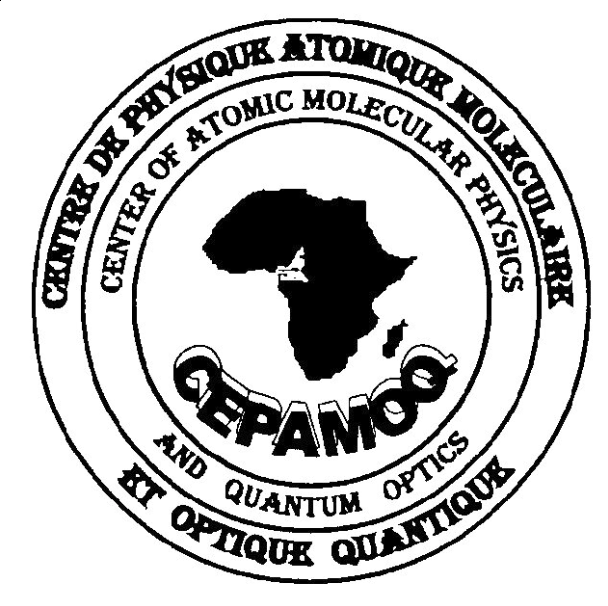
\includegraphics[scale=.10]{cepamoq.png}
\end{textblock*}


\begin{textblock*}{270pt}(325pt,100pt)
 
\includegraphics[scale=.25]{anbg.jpg}
\end{textblock*}

%\begin{textblock*}{270pt}(200pt,60pt)
% 
\includegraphics[scale=.50]{Universite-de-Douala.png}
%\end{textblock*}

% \begin{itemize}
%   \item Logo USTM
%   \item Logo CEPAMOQ
%   \item Logo ANBG
% \end{itemize} 
\end{frame}
